\documentclass[20pt]{extarticle}
\usepackage[landscape]{geometry}
\usepackage{fontspec}
\usepackage{graphicx}

\usepackage[xetex, bookmarks, colorlinks, breaklinks]{hyperref}
\hypersetup{linkcolor=blue,citecolor=blue,filecolor=black,urlcolor=blue} 
\usepackage[usenames,dvipsnames]{color}
\setmainfont{Fontin}
\pagestyle{empty}

\newcommand{\cmr}{\fontencoding{T1}\fontfamily{cmr}\selectfont} % Computer Modern Roman

\begin{document}
\begin{center}

\vspace*{\fill}


{\fontsize{40}{40} \sc Hosting Queryable and Highly Available Linked Data for Free}\\

\vspace{10 mm}

{\cmr Luca Matteis \href{https://twitter.com/lmatteis}{@lmatteis}}
\\
{\cmr Ruben Verborgh \href{https://twitter.com/RubenVerborgh}{@RubenVerborgh}}

\vspace*{\fill}
\end{center}

\newpage

\begin{center}
{\fontsize{35}{35}\color{blue} \sc Motivation 1}
\end{center}

\vspace{10 mm}

{\fontsize{30}{30} {\cmr 
\noindent SPARQL endpoints require the need to \\{\color{blue}buy and configure complex servers}.
\\ \\
You need to worry about: 

- having the funds to keep the server running

- making sure the system is up-to-date

- many other sys-admin tasks
\\ \\
{\color{blue} 
\textbf{\textit{TL;DR}}

Hosting an RDF file is a lot easier than hosting a SPARQL endpoint. 
}
}}

\newpage
 
 
\begin{center}
{\fontsize{35}{35}\color{blue} \sc Motivation 2}
\end{center}

\vspace{10 mm}

{\fontsize{30}{30} {\cmr 
\noindent SPARQL endpoints {\color{blue}suffer from low-availability.}
\\ \\
They offer consumers the ability to run any query they want. Therefore consumers will run any query they want and will quickly overload the server with too many complex requests.
}
\vspace{10 mm}
\begin{figure}[ht!]
\centering
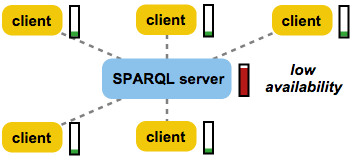
\includegraphics[width=110mm]{sparql.png}
\end{figure}



\newpage

 \begin{center}
{\fontsize{35}{35}\color{blue} \sc Problem}
\end{center}

\vspace{10 mm}

{\fontsize{30}{30} {\cmr 
\noindent {\color{blue} Hosting SPARQL endpoints requires too much effort}, both in terms of cost and server maintenance.
\\ \\
Fortunately SPARQL endpoints are not the only way of publishing queryable Linked Data.
\\ \\
\textit{Triple Pattern Fragments} is a way of publishing queryable Linked Data on low cost servers.
}} 

\newpage


\begin{center}
{\fontsize{35}{35}\color{blue} \sc LDstatic \& LDF-GAE}
\end{center}
\vspace{20 mm}
{\fontsize{30}{30} {\cmr 
\noindent We have developed two tools, LDstatic \& LDF-GAE, that implement the \textit{TPF} protocol on low cost servers.
\\ \\
{\color{blue} 
\textbf{\textit{TL;DR}}

Users can run SPARQL queries against Linked Data published on online file repositories and cloud hosting services such as \textbf{GitHub}, \textbf{Google Code}, \textbf{Google App Engine} or \textbf{Dropbox}.
}
}} 


\newpage

\begin{center}
{\fontsize{35}{35}\color{blue} \sc LDstatic}
\end{center}
\begin{figure}[ht!]


\includegraphics[width=50mm]{GitHub.jpg}
\end{figure}
\vspace{5 mm}
{\fontsize{30}{30} {\cmr 
\noindent \textbf{GitHub Pages}, and other online file repositories, can serve static HTML files.
\\ \\
It can also serve other type of content, such as N-Triples (\texttt{.nt}).
\\ \\
This means that GitHub Pages can serve triple pattern fragments.
}} 


\newpage

\begin{center}
{\fontsize{35}{35}\color{blue} \sc LDstatic}
\end{center}
\vspace{10 mm}
{\fontsize{30}{30} {\cmr 
\noindent We want to match\\\\
\texttt{<foo> <bar> "literal" .}\\\\
using: \\\\
\texttt{/?subject=<foo>}\\
\texttt{/?predicate=<bar>}\\
\texttt{/?object="literal"}\\
\texttt{/?subject=<foo>\&predicate=<bar>}\\
\dots
\\\\
We need at least 8 static files for each triple if we want to match all combinations.
}} 

\newpage

\begin{center}
{\fontsize{35}{35}\color{blue} \sc LDstatic}
\end{center}
\vspace{10 mm}
{\fontsize{30}{30} {\cmr 
\noindent Having all combinations is important for triple pattern fragments \textit{enabled} clients so they can run complex queries, even SPARQL queries!
\\\\
So we can host queryable linked data on GitHub Pages:
\begin{center}
\url{http://lmatteis.github.io/ldstatic/}
\end{center}
}} 



\newpage

\begin{center}
{\fontsize{35}{35}\color{blue} \sc LDF-GAE}
\end{center}
\vspace{10 mm}
\begin{figure}[ht!]
\centering

\includegraphics[width=40mm]{appengine-logo.png}
\end{figure}
{\fontsize{30}{30} {\cmr 
\noindent Now we talk about our other TPF implementation, which lets us run SPARQL queries on {\color{blue}Google App Engine}.

\begin{center}
\url{http://ldf-gae.appspot.com/}
\end{center}

Instead of static files we use their native APIs to store and retrieve triples.
}} 


\end{document}